\chapter{Design-Dokument}
\section{Einleitung}
Dieses Dokument dient der Darstellung der Gesamt-Architektur des Software-Projekts "Freya-MPD-Client"
Zuerst wird das grundsätzliche Problem beschrieben und anschließend mit entsprechenden Beispielen und
UML-Diagrammen erläutert.\ \\
Im Anschluss daran wird die Benutzeroberfläche präsentiert und in Bereiche aufgeteilt genauer dargestellt.
Dabei werden alle Schaltflächen und Info-Panel genau erläutert.
Anschließend folgt eine Übersicht zu allen Short-Cuts die genutzt werden können.
Danach werden einige Use-Case-Fälle angeschaut, um genau zu verstehen, wie die Software mit dem Nutzer
interagiert und auf Befehle reagiert.
\newpage
\section{Hauptproblem}
Der Freya-MPD-Client muss Kommandos an den MPD-Server senden (z.B. Play, Stop, etc.) und  gleichzeitig auf 
Änderungen reagieren können (z.B. Änderung der Lautstärke), da auch andere MPD-Clients sowie der Server
selbst unabhängig Änderungen vorhnehmen können. Diese Änderungen muss der MPD-Client an andere Programmteile
weiterleiten können (Observer Pattern).\ \\
Solange der Server nicht aktiv ist, sollte er keinerlei Hardwareressourcen verbrauchen. Der MPD-Client sollte
nach Möglichkeit Verbindung zu einem Server aufbauen und auch wieder trennen können, diese Änderungen müssen
natürlich wieder an andere Programmteile weitergeleitet werden (Observer Pattern).\ \\
Das MPD-Protokoll \footnote{http://www.musicpd.org/doc/protocol/index.html} bietet zwei Möglichkeiten, dies zu 
realisieren.\ \\ \\
\textbf{Möglichkeit 1:}\ \\ \\
Periodisch (z.B. alle 500ms) das Kommando 'status', und nach Bedarf Kommandos wie z.B. 'currentsong' absetzen.
Das Problem dabei ist allerdings, dass es unnötig viel Netzwerk-Traffic erzeugt und für langsame Internetanbindungen
somit zur Belastung wird. Dies ist allerdings eine gängige Methode, wenn es z.B. darum geht sekündlich die 
Netzwerkübertragungsrate anzuzeigen.\ \\ \\
\textbf{Möglichkeit 2:}\ \\ \\
Die zweite Möglichkeit ist die Nutzung der 'idle' und 'noidle' Kommandos. 'idle' verstzt die die Verbindung zum Server
in einen Schlafzustand, sobald nun Ereignisse wie z.B. 'player' (Play, Pause, etc.) eintreten, wacht diese Verbindung
aus dem Schlafzustand auf und sendet an den Client eine Liste der Ereignisse die eingetroffen sind.
Es gibt allerdings eine Einschränkung:\ \\
Während die Verbindung im 'idle' Modus ist, kann kein reguläres Kommando wie z.B. 'play' gesendet werden, da der 
Server ansonsten die Verbindung zum Client trennt. Die einzige Möglichkeit aus dem 'idle' Modus zu wechseln, ist
das 'noidle' Kommando abzusetzen, während die Verbindung schläft. Jedoch gibt es auch hier ein Problem, denn das
'idle' Kommando blockiert, wir wollen allerdings in der Wartezeit dennoch eine bedienbare grafische Oberfläche.\ \\
Prinzipiell gibt es drei Möglichkeiten dieses Problem zu lösen:\ \\ \\
\textbf{Möglichkeit 1:}\ \\ \\
Man hält zwei Verbindungen zum Server, eine die Kommandos sendet und eine die sich stets im 'idle' Modus befindet.
Für die Realisierung müssten Threads herangezogen werden. Ein Thread, würde im Hintergrund nach Ereignissen lauschen.
Problem: Es müssten zwei Verbindungen abgehandelt werden, was wiederum ein Mehraufwandt an Code bedeutet. Des weiteren
werden Threads benötigt, die wiederum in anderen Bereichen des Programms Lockingmechanismen hervorufen würden.\ \\ \\
\textbf{Möglichkeit 2:}\ \\ \\
Man hält eine asynchrone Verbindung zum Server. Diese kann das 'idle' Kommando zum Server schicken, returned aber sofort.
Um nun eine Liste der Ereignisse zu bekommen, setzt man einen \"Watchdog\" auf die asynchrone Verbindung an. Hierfür wird
Glib::signal\_io() benutzt, dass sich in den laufenden MainLoop \footnote{Gtk+ benutzt intern einen MainLoop um auf die 
Benutzer-Eingaben reagieren zu können. Desweiteren kann man eigene Events in den Loop einhängen, wie z.B. ein Timeoutereigniss,
das alle 500ms ausgeführt wird.} einhängt und eine Callbackfunktion aufruft sobald auf der Verbindung etwas interessantes 
passiert.\ \\ \\
\textbf{Praktische Darstellung:}\ \\ \\
Zum parktischen Verständnis kann man eine Telnet-Session zum Server aufbauen:
\begin{itemize}
	\item Trying ::1...
	\item Connected to localhost.
	\item OK MPD 0.16.0 (Der Server antwortet bei Verbindungsaufbau stets mit einem OK und der Versionsnummer)
	\item pause (Wir senden das 'pause' Kommando zum pausieren des aktuellen Liedes)
	\item OK (Der Server führt es aus und antwortet mit einem OK)
	\item play (Wir senden das 'play' Kommando zum abspielen des aktuellen Liedes)
	\item OK (Der Server führt es aus und antwortet mit einem OK)
	\item idle (Wir sagen dem Server, dass wir die Verbindung schlafen legen wollen)
	\item changed:player (Der Server returned allerdings sofort, da seit dem Verbindungsaufbau etwas geschehen ist)
	\item changed:mixer (Und zwar wurde der Player pausiert, und die Lautstärke geändert)
	\item OK (Das Ende des idlemodes wird wieder mit OK angezeigt)
	\item idle (Wir sagen dem Server, dass wir die Verbindung schlafen legen wollen, er antwortet nicht mit OK sondern schläft jetzt.
Würden wir in einem anderen Client pausieren, so würde er hier aufwachen)
	\item noidle (Um aus dem 'idle' Modus vorher aufzuwachen, senden wir das 'noidle' Kommando)
	\item OK (Ok sagt uns, dass alles gut gelaufen ist)
	\item idle (Probieren wir einmal ein Kommando zu senden während die Verbindung schläft)
	\item play (zum Beispiel das 'play' Kommando, als antwort wird die Verbindung getrennt)
	\item Connection closed by foreign host.
\end{itemize}
Die Idee zu dieser Implementierung (speziell das Benutzen einer asynchronen Verbindung), kommt von 'ncmpc' \footnote{http://mpd.wikia.com/wiki/Client:Ncmpc},
der inoffiziellen offiziellen Referenzimplementierung des MPD, Author Max Kellermann.
\section{Softwarearchitektur}
\subsection{Architekutrübersicht}
\subsubsection{Namespace-Übersicht}
\begin{figure}[h]
\centering
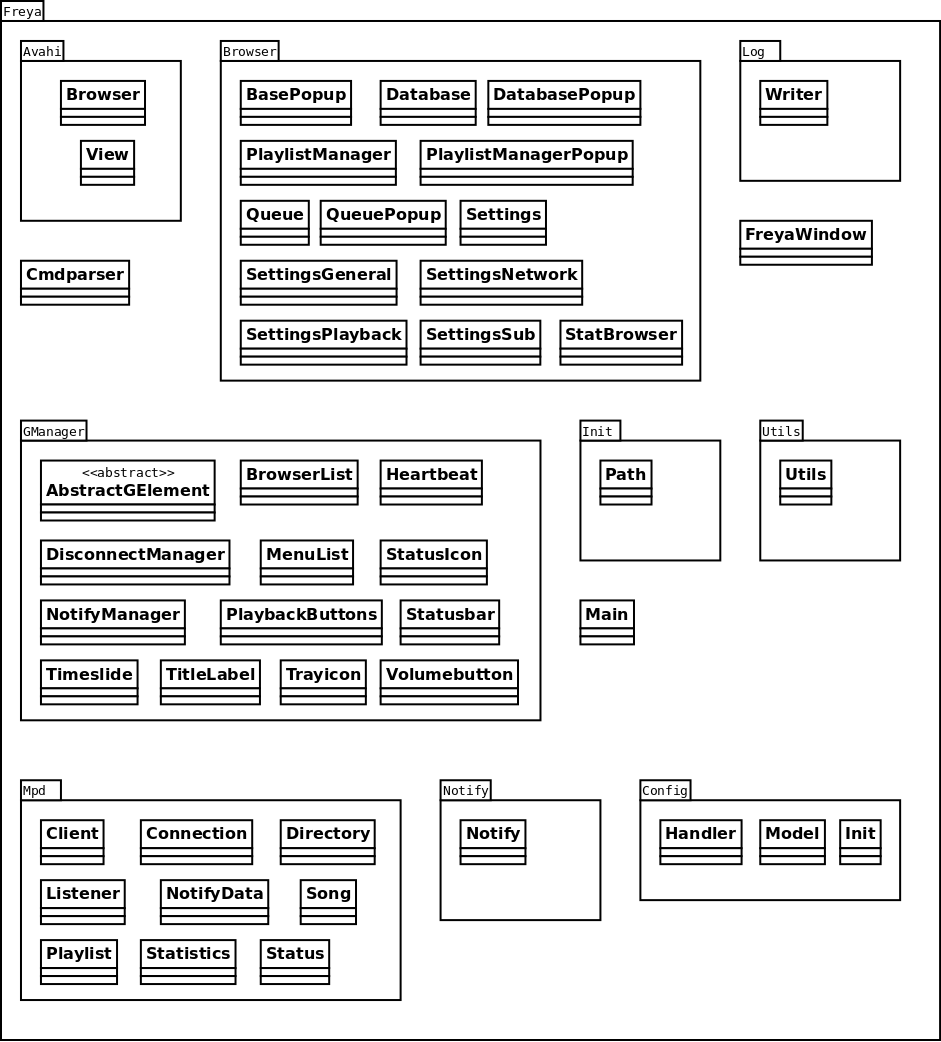
\includegraphics[scale=0.3]{Namespace_Uebersicht.png}
\end{figure}
\newpage
\subsubsection{Beschreibung}
\subsection{Funktionen}
\subsubsection{Beispiel-Abspielfunktionen}
\subsubsection{Beispiel-Playlist erstellen}
\subsubsection{Beispiel-Dateibrowser}
\subsection{Oberfläche}
\subsubsection{Titelleiste}
\subsubsection{Seitenmenü}
\subsubsection{Fußleiste}
\subsubsection{Anzeige}
\subsection{Short-Cuts}
\section{Use-Case-Fälle}
\subsection{Musik abspielen}
\subsection{Musik zufällig abspielen}
\subsection{Musik im Consume Mode abspielen}
\subsection{Playlist erstellen}

